\documentclass[../../main.tex]{subfiles}

\begin{document}
\section{Considerazioni sulla dashboard del DPC}
Apriamo questa sezione riportando uno screenshot della dashboard del DPC effettuato in data 17 febbraio '21.

\begin{figure}[h]
    \centering
    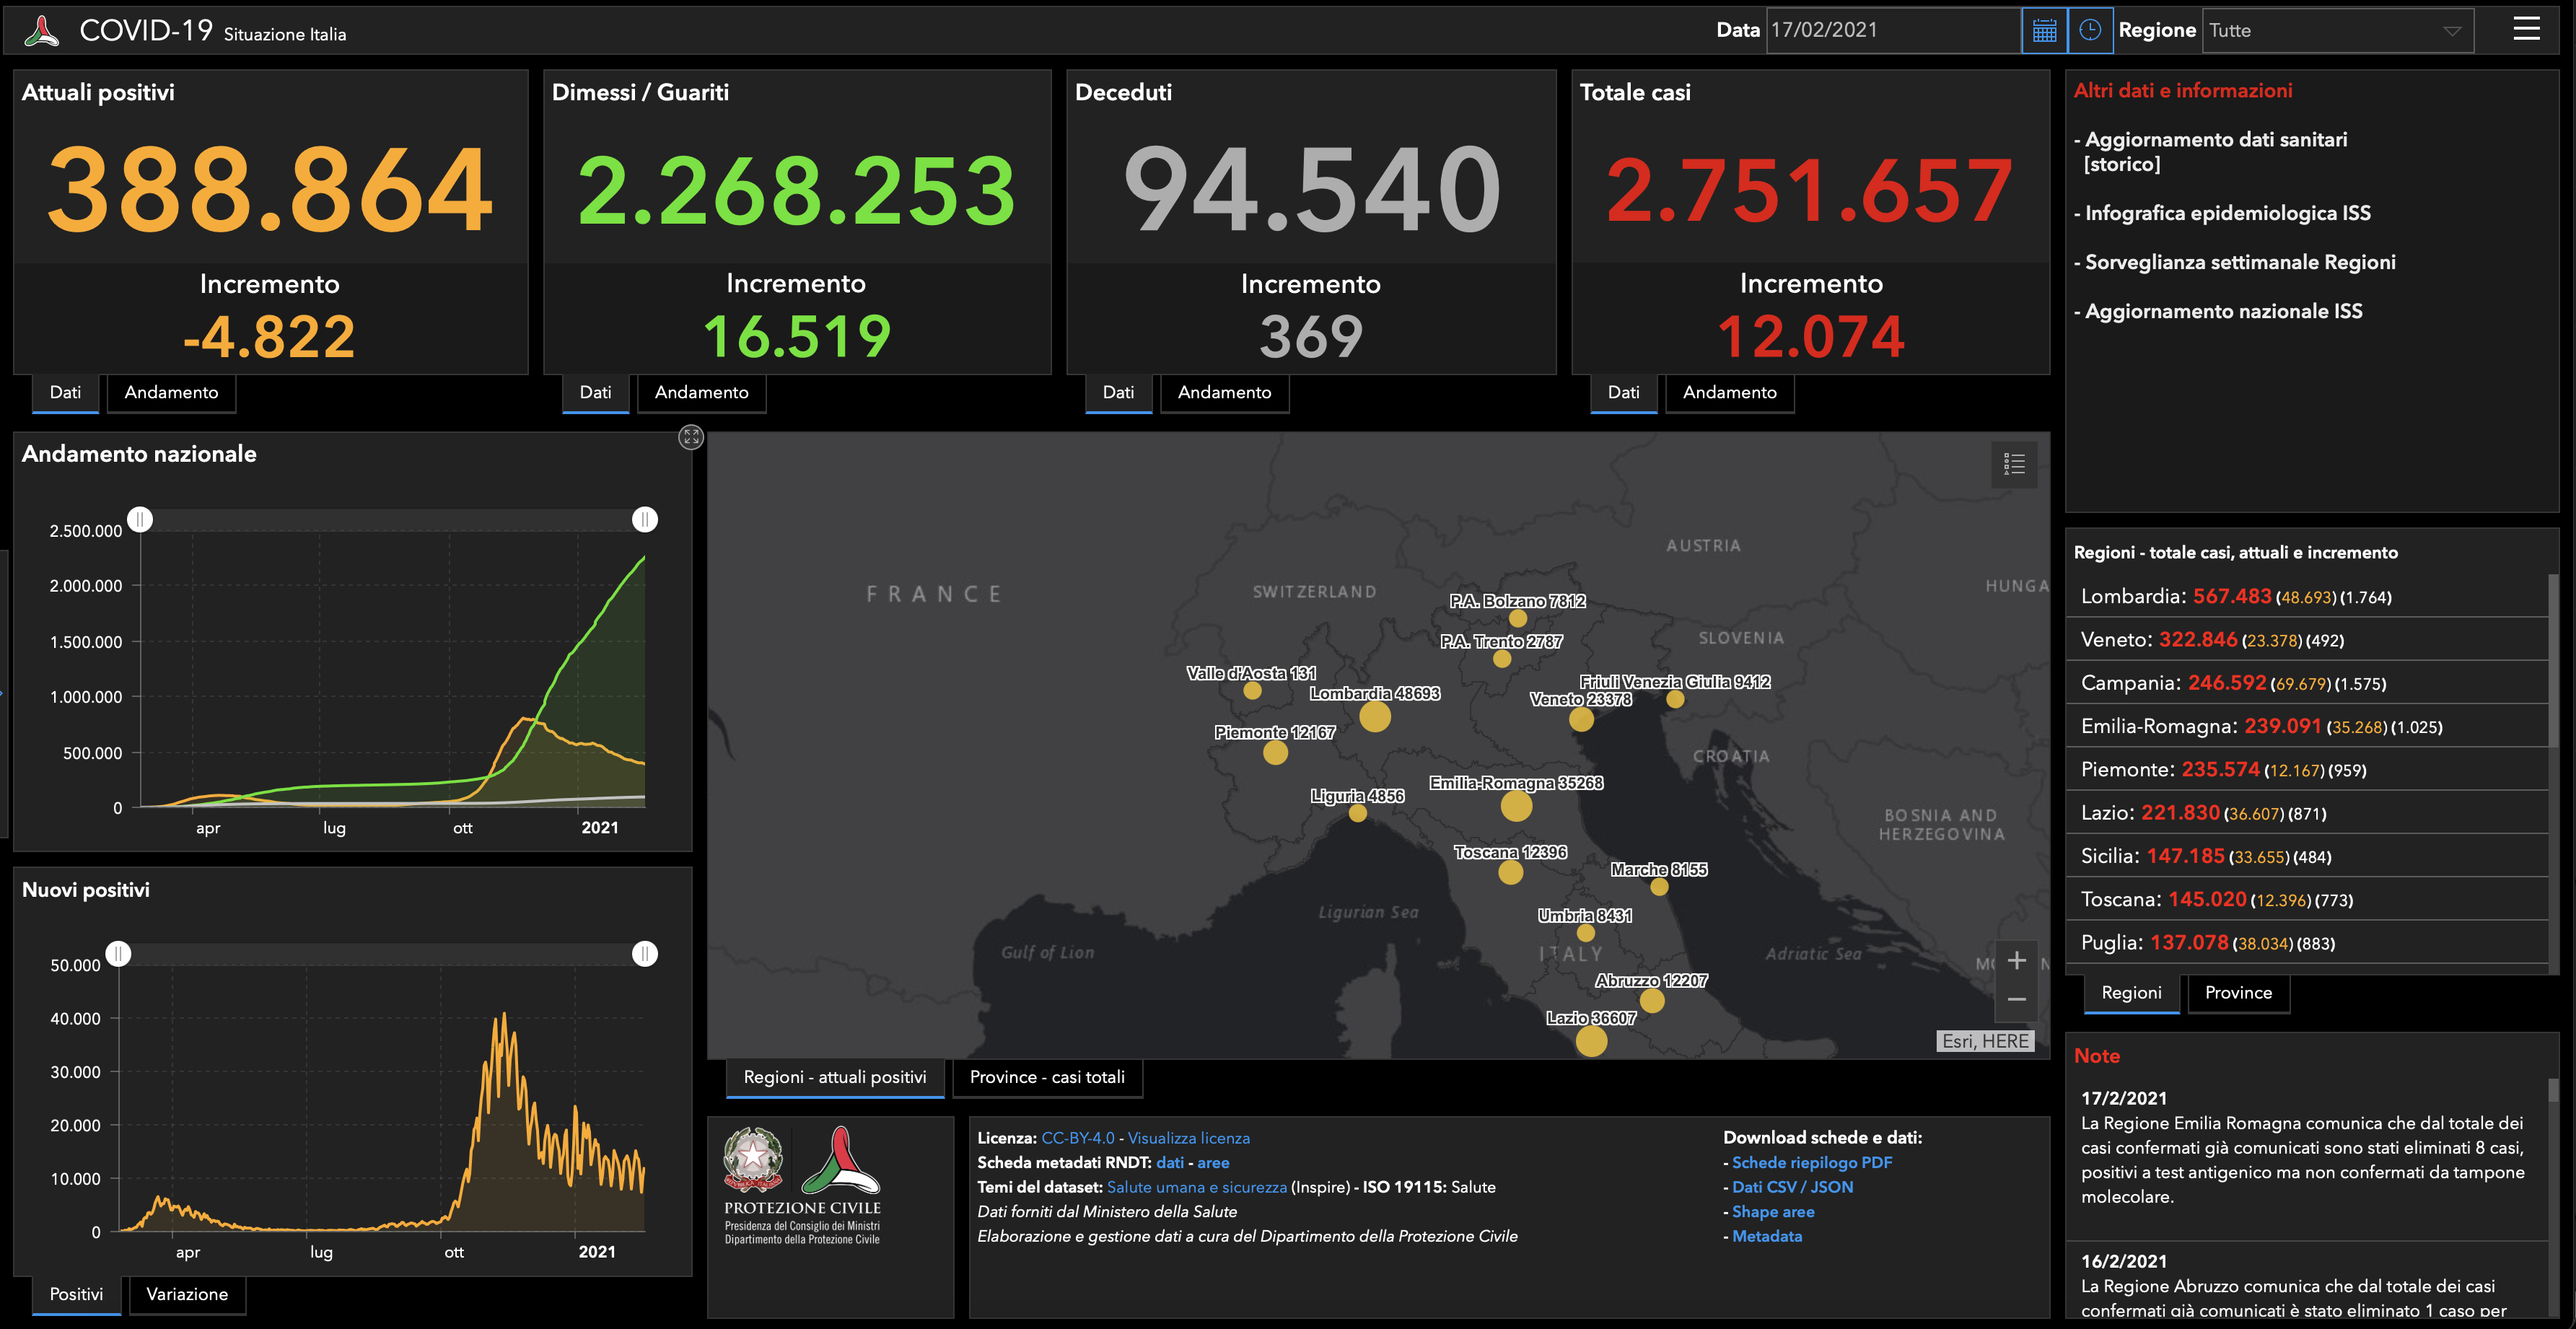
\includegraphics[width = \textwidth]{screenshot-dashboard-DPC}
    \caption{Screenshot della dashboard del Dipartimento della Protezione Civile catturato in data 17 febbraio '21.}
    \label{fig:screen-dashboard-DPC}
\end{figure}

Di seguito riportiamo le principali criticità riscontrate articolandole in due parti: la prima si riferisce agli aspetti estetici e strutturali che minano l'usabilità complessiva e concorrono ad una scadente esperienza utente, mentre la seconda attiene alle carenze nel contenuto informativo e nelle funzionalità che ne riducono il raggio di utilità.

\subsection{Criticità nell'esperienza utente}
\begin{enumerate}
    \item Dimensione eccessivamente piccola di alcune scritte: il riferimento è ai due box in basso a quello in alto della parte destra dell'interfaccia, il cui contenuto è difficilmente leggibile, specie se la dashboard viene consultata su dispositivi con schermi ridotti;
    \item Inconsistenza nel riempimento dei box: il riferimento è alla differente densità del contenuto tra il box in alto e quello in basso della parte destra dell'interfaccia, il che si traduce in un utilizzo inefficiente dello spazio disponibile a svantaggio di altre componenti grafiche che, conseguentemente, risultano troppo piccole;
    \item Distanza dal modello mentale degli utenti nell'interazione con la mappa: se l'utente clicca sull'area di una regione gli vengono restituiti inutili codici identificativi della stessa, mentre qualora clicca sul cerchio giallo che la contrassegna, gli vengono presentati i valori delle metriche epidemiologiche; questo differente comportamento disorienta l'utente, il quale, stando al classico modello mentale, si aspetterebbe un feedback consistente a fronte delle sue due simili interazioni;
    \item Discrepanza tra significante\footnote{Per \textit{significante} si intende }  e comportamento effettivo: il riferimento è alla lista delle regioni presente nella parte centrale destra dell'interfaccia, le cui singole righe sono cliccabili come suggerito dalla comparsa della manina quando vi si pone il cursore, tuttavia al click non segue alcuna applicazione di filtri sui dati, come invece l'utente si aspetterebbe;
    \item Mancanza di prevenzione degli errori nel widget calendario: il widget del calendario preposto all'inserimento della data rispetto cui vedere i dati permette all'utente di inserire anche date future, per le quali, comprensibilmente, l'interfaccia non visualizza alcunché;
    \item Interazione limitata con la mappa: l'utente può esclusivamente gestire lo zoomdella mappa, mentre sono del tutto assenti altri controlli relativi, a mo' d'esempio, al reset della visualizzazione di default ovvero alla geolocalizzazione dell'utente stesso, entrambe funzionalità che migliorerebbero notevolmente l'esperienza d'uso;
    \item Assenza di componenti grafiche per ridurre carico cognitivo: l'interfaccia non fa uso di icone atte a catturare l'attenzione del lettore al fine di semplificargli l'individuazione delle metriche di interesse, costringendolo a leggere attentamente ogni etichetta;
    \item Adozione del colore come unico mezzo distintivo delle componenti: il riferimento è ai link presenti nella parte bassa dell'interfaccia, i quali non presentano la sottolineatura che è essenziale per coloro che han difficoltà visive, nonché ai link presenti in alto a destra che non presentano né il colore blu tantomeno la sottolineatura;
    \item Difficoltà dell'interazione coi grafici: le curve dei grafici dell'inche posizioni il cursore esattamente sulla curva di interesse, il che, specie su schermi piccoli, si traduce in una notevole difficoltà nel completare questa interazione;
\end{enumerate}

\subsection{Criticità nella capacità informativa}
Abbiamo condotto svariati test sull'interfaccia della dashboard in oggetto ed è risultata carente oltre che nelle funzionalità atte ad una maggiore contestualizzazione e confrontabilità dei dati anche nella comunicazione di determinate informazioni di particolare significatività.
Per quanto riguarda le funzionalità assenti e ritenute di estrema utilità dai giornalisti prestatisi ai test, certamente si può annoverare la possibilità di confrontare l'andamento del quadro epidemiologico tra due regioni e/o tra due periodi temporali; ancora, significativa sarebbe la funzionalità tramite cui i giornalisti potrebbero studiare la distribuzione delle metriche epidemiologiche su variabili anagrafiche, come l'età, i genere, l'impiego.
Mentre, relativamente alle informazioni non comunicate e che costringono i giornalisti a rivolgersi a differenti fonti, rientrano il numero dei tamponi, le disponibilità totali delle strutture ospedaliere, nonché gli innumerevoli indicatori aggregati quali il tasso di positività, il tasso di letalità, il tasso di occupazione delle terapie intensive, la normalizzazione delle metriche sulla popolazione.

\end{document}